% Replace the existing figure with label fig:fdr in:
% docs/ICSPS2026_LaTeX/ICSPS2026_paper.tex
% Paths below assume compilation from docs/ICSPS2026_LaTeX.
% The manuscript must load graphicx, as the current draft does.
% Keep the natural aspect ratio; do not retain the old 1.15in placeholder height.
\begin{figure}[!t]
  \centering
  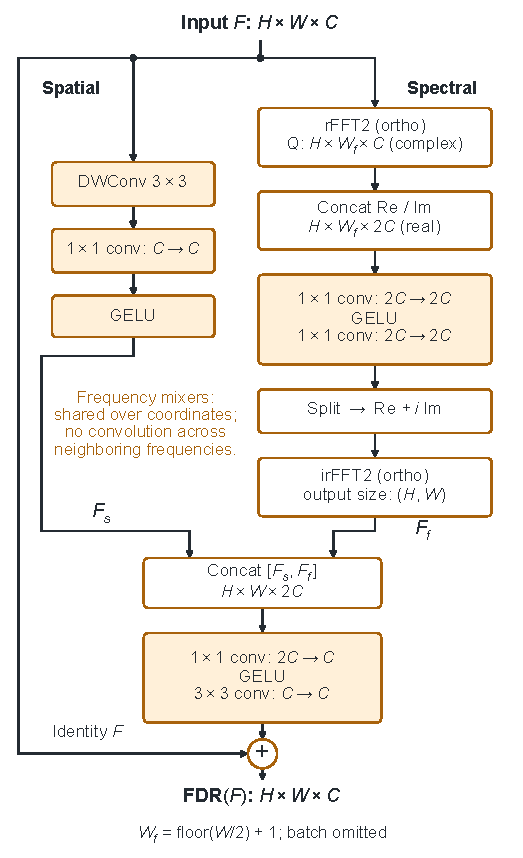
\includegraphics[width=\columnwidth]{../../output/pdf/ICSPS2026_Fig2/fig2_fdr_block.pdf}
  \caption{Full-spectrum Fourier residual refinement (FDR). A depthwise--pointwise spatial branch complements a spectral branch. The one-sided rFFT representation retains all nonredundant frequencies. Shared real-valued \(1\times1\) convolutions mix channels and real--imaginary components independently at each frequency coordinate, without convolution across neighboring frequencies. After inverse rFFT, spatial and spectral features are concatenated, projected, and added to the input.}
  \label{fig:fdr}
\end{figure}
